\documentclass[lang=cn, device=normal, color=blue, titlestyle=hang, scheme=english, mode=fancy, citestyle=gb7714-2015, bibstyle=gb7714-2015, toc=onecol, 11pt]{elegantbook}
\setcounter{tocdepth}{1}
\ExecuteBibliographyOptions{sorting=gb7714-2015}

\usepackage{listings}
\usepackage{accsupp}

\newcommand{\emptyaccsupp}[1]{\BeginAccSupp{ActualText={}}#1\EndAccSupp{}}

\definecolor{typecolor}{HTML}{2B91AF}
\definecolor{funccolor}{HTML}{74531F}
\definecolor{macrocolor}{HTML}{8A1BFF}
\lstset{
	tabsize = 4,
	columns = fixed,
	numbers = left,
	breaklines = true,
	keywordstyle = \color[RGB]{40,40,255},
	numberstyle = \scriptsize\color{darkgray}\emptyaccsupp,
	basicstyle = \normalsize\ttfamily,
	commentstyle = \normalsize\color[RGB]{0,128,0},
	stringstyle = \normalsize\slshape\color[RGB]{128,0,0},
	showstringspaces = false,
}
\lstdefinelanguage[17]{C++}[11]{C++}{
	morekeywords={%
		},
	emphstyle=\color{typecolor},
	moreemph={%
		},
	emphstyle={[2]\color{funccolor}},
	moreemph={[2]%
			main,%
		},
	emphstyle={[3]\color{macrocolor}},
	moreemph={[3]%
		},
}


\usepackage{zhlipsum}

\title{上手 CMake}
\subtitle{Shangshou CMake}
\date{\today}
\author{UnnamedOrange}
\version{开发版}

\extrainfo{Licensed under the Creative Commons Attribution Share Alike 4.0 International.}
\cover{cover}

\begin{document}

	\maketitle

	\chapter*{前言}
	\markboth{前言}{前言}

	% Licensed under the Creative Commons Attribution Share Alike 4.0 International.
% See the LICENSE file in the repository root for full license text.

这是前言。请在源代码中修改 License 说明。请使用 Xe\LaTeX 编译。


	\tableofcontents

	\mainmatter

	% Licensed under the Creative Commons Attribution Share Alike 4.0 International.
% See the LICENSE file in the repository root for full license text.

\chapter{安装并使用 CMake}


% Licensed under the Creative Commons Attribution Share Alike 4.0 International.
% See the LICENSE file in the repository root for full license text.

\section{从官网上获取资源}

一般而言,前往官网下载软件资源是最好的选择。在搜索引擎搜索 CMake,发现其官网为 \url{https://cmake.org}。点击官网页面右上角的 Download 链接进入下载页面,在二进制分发文件(Binary distributions)中下载适合自己系统的 CMake。对于一般的 Windows 用户,下载 x64 安装包(Windows x64 Installer)即可。安装过程中需注意,请选择将 CMake 添加到系统 PATH 环境变量中,如图 \ref{fig:cmake-installment} 所示。

\begin{figure}[H]
	\centering
	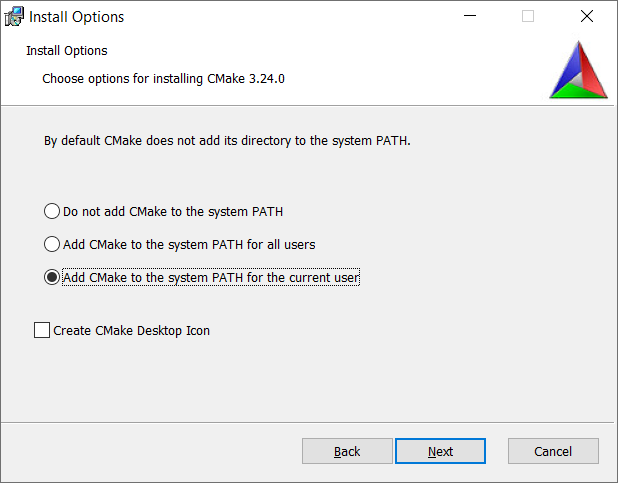
\includegraphics[width=0.6\linewidth]{assets/cmake-installment}
	\caption{安装 CMake 时,请选择添加 CMake 到系统 PATH 环境变量中。}
	\label{fig:cmake-installment}
\end{figure}

Linux 用户无需参考本文中关于软件安装与命令行使用的内容。但需要注意,不同 Linux 发行版附带的 CMake 版本不同,往往不是最新版本。

在官网页面右上角的链接中还能找到 CMake 的官方文档:\url{https://cmake.org/cmake/help/latest/}。它只能作为细则的参考,无法作为一份教程去学习——尽管其中附有一份教程\footnote{网址:\url{https://cmake.org/cmake/help/latest/guide/tutorial/index.html}。},但其质量不足以让你真正掌握 CMake,其中的部分内容也稍有过时。


% Licensed under the Creative Commons Attribution Share Alike 4.0 International.
% See the LICENSE file in the repository root for full license text.

\section{通过 GUI 使用 CMake}

安装的 CMake 附带了一个\emph{图形用户界面(graphics user interface,GUI)}应用程序,名为 cmake-gui。从开始菜单依次打开“CMake”“CMake (cmake-gui)”,将显示图 \ref{fig:cmake-gui-1} 所示的窗口。

\begin{figure}
	\centering
	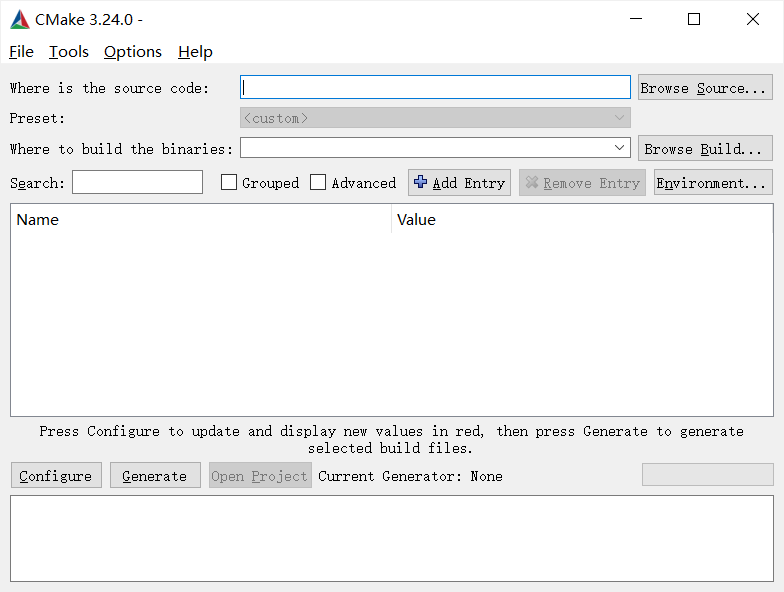
\includegraphics[width=0.6\linewidth]{assets/cmake-gui-1}
	\caption{cmake-gui 程序的窗口。}
	\label{fig:cmake-gui-1}
\end{figure}

图 \ref{fig:cmake-gui-2} 解释了该窗口中各部分的含义。图中最抢眼的是中间的列表控件,它被称为\emph{缓存变量(cached variable)}列表。缓存变量将允许我们自定义项目的一些选项。CMake 将缓存变量的值保存在生成的一个临时文件 \lstinline[language={}]{CMakeCache.txt} 中,我们可以借助 cmake-gui 的这个列表控件方便地修改它们。一般而言,一旦缓存变量文件被生成,缓存变量的值就不会随 CMake 的运行而改变,它们将一直采用缓存变量文件保存的值:所以在之后的实验过程中,如果总是出现未知的错误,不妨删除 \lstinline[language={}]{CMakeCache.txt} 后再试一次。

\begin{figure}
	\centering
	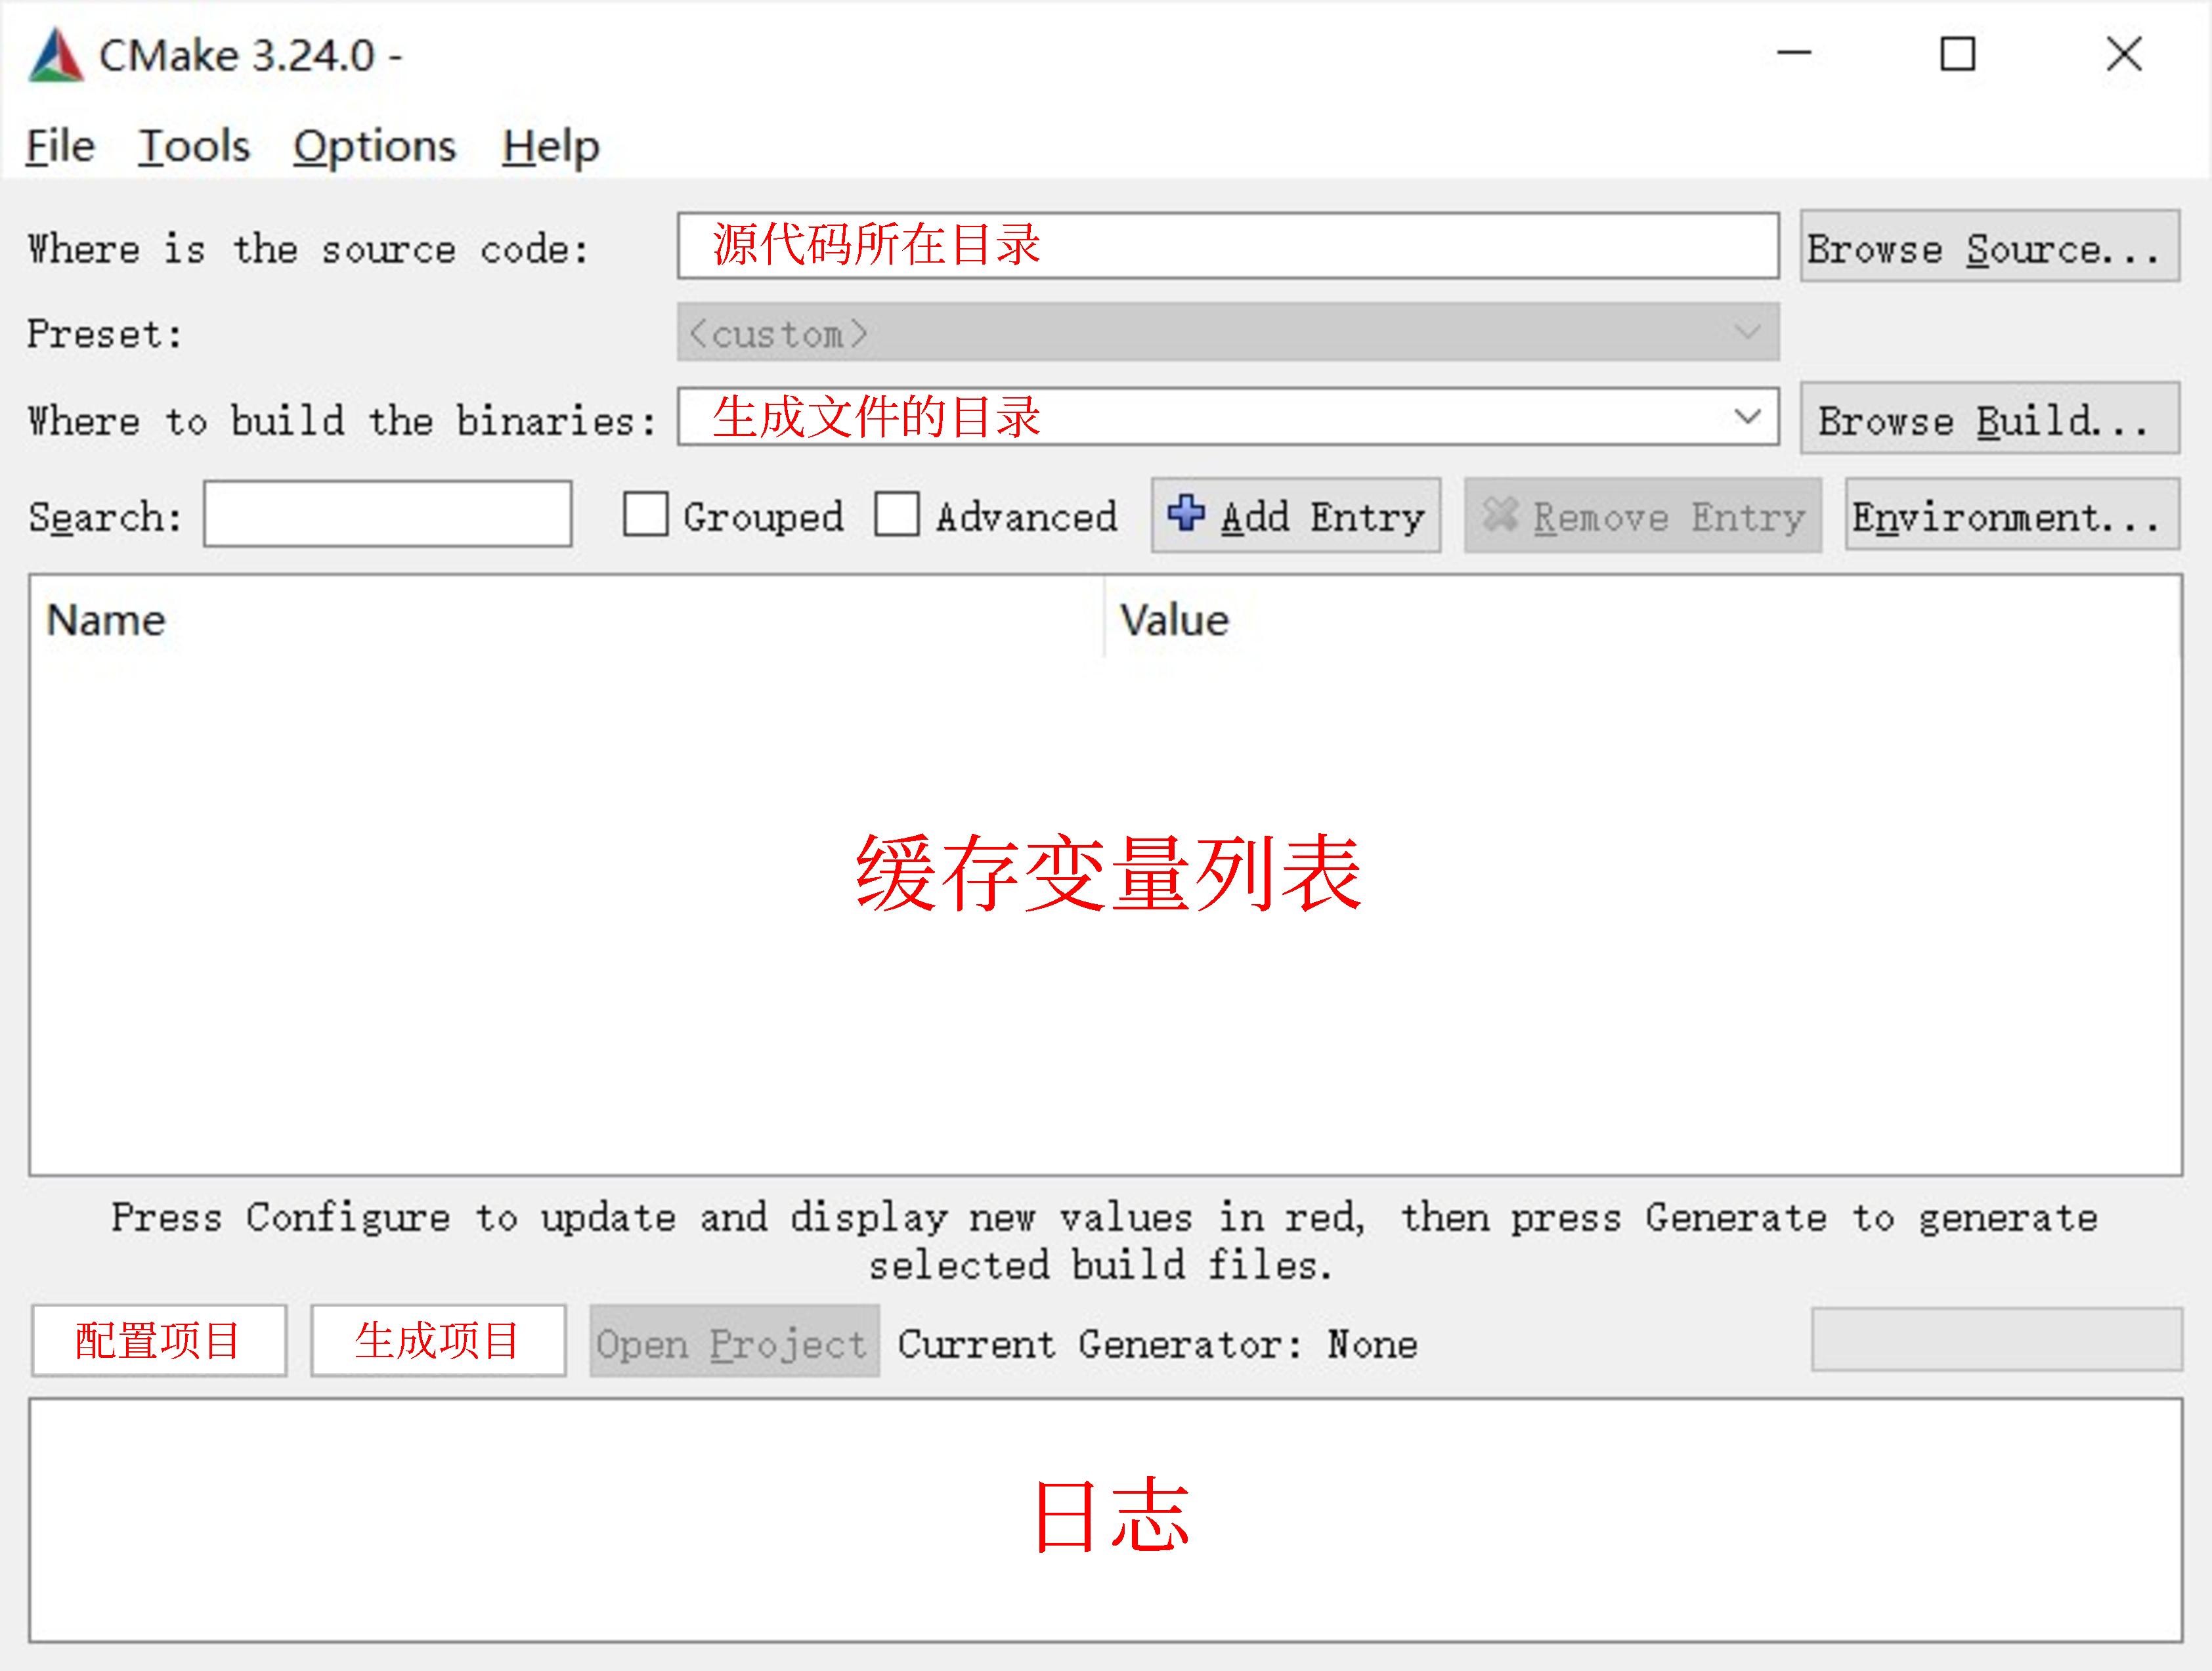
\includegraphics[width=0.6\linewidth]{assets/cmake-gui-2}
	\caption{cmake-gui 窗口解释。}
	\label{fig:cmake-gui-2}
\end{figure}

% TODO: 把“下一章”替换为“第 n 章”,其他同理。

我们将在下一章中详细讲解缓存变量的相关知识。除了配置缓存变量这一功能,cmake-gui 还能帮助我们调用真正的 CMake 程序,对应图 \ref{fig:cmake-gui-2} 中的“配置项目”“生成项目”按钮,我们将在下一节讲解它们的作用。由于 cmake-gui 的本质是帮助我们修改文本文件、调用命令行,而市面上的大量 IDE 都已很好地集成了 CMake,所以在开发时和自动化测试时我们一般都不使用 cmake-gui。cmake-gui 一般只用于刚刚从网络上下载的项目,这时它相比命令行可谓简而不繁。


% Licensed under the Creative Commons Attribution Share Alike 4.0 International.
% See the LICENSE file in the repository root for full license text.

\section{CMake 的基本工作流程}


% Licensed under the Creative Commons Attribution Share Alike 4.0 International.
% See the LICENSE file in the repository root for full license text.

\section{通过命令行使用 CMake}


% Licensed under the Creative Commons Attribution Share Alike 4.0 International.
% See the LICENSE file in the repository root for full license text.

\section{通过 IDE 使用 CMake}


% Licensed under the Creative Commons Attribution Share Alike 4.0 International.
% See the LICENSE file in the repository root for full license text.

\begin{problemset}
	\item 简述包含一个源文件(\lstinline[language={}]{.cpp})和若干头文件的可执行文件项目的生成流程。

	\item 阅读下面的 C++ 程序。

	\begin{lstlisting}[language={[latest]C++}, moreemph={[2]foo}]
void foo();

int main()
{
	foo();
	bar();
}
	\end{lstlisting}

	不使用编译器,说明这个程序会报出的编译错误。假设该程序的编译错误已被修复,说明该程序将会报出的链接错误。
\end{problemset}



\end{document}
